\documentclass[tikz,border=3.14mm]{standalone}

\begin{document}
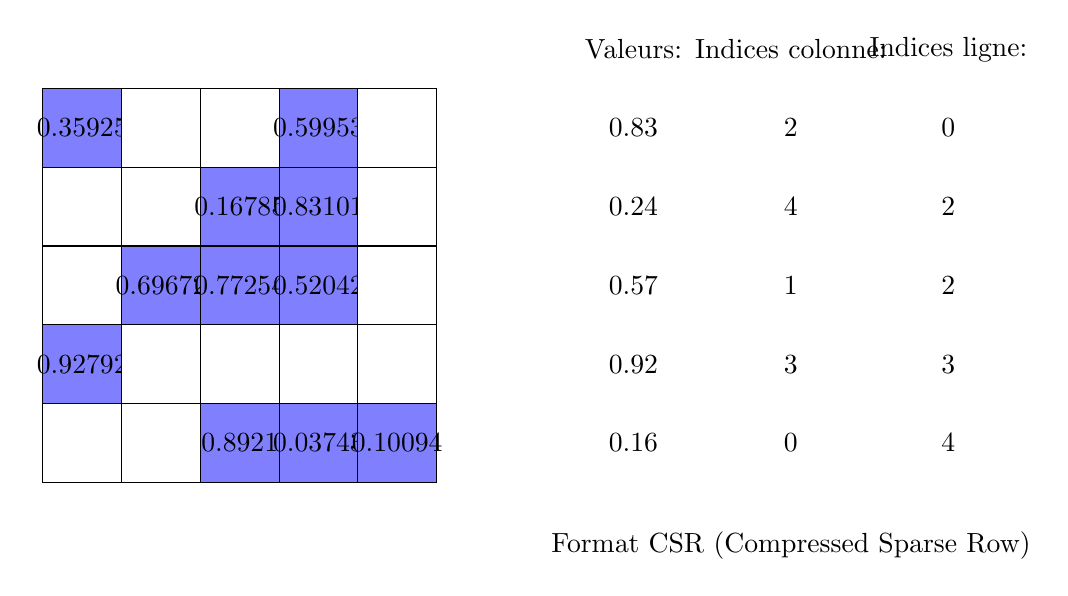
\begin{tikzpicture}

% Draw the matrix
\foreach \x in {0,...,4} {
    \foreach \y in {0,...,4} {
        \pgfmathsetmacro{\rand}{rnd}
        \ifdim \rand pt < 0.7pt % 70% zeros
            \draw[fill=white] (\x, \y) rectangle (\x+1, \y+1);
        \else
            \draw[fill=blue!50] (\x, \y) rectangle (\x+1, \y+1);
            \node at (\x+0.5, \y+0.5) {\pgfmathparse{rnd}\pgfmathresult};
        \fi
    }
}

% Draw the compressed representation
\begin{scope}[xshift=7cm]
\node at (0.5, 5.5) {Valeurs:};
\node at (0.5, 4.5) {0.83};
\node at (0.5, 3.5) {0.24};
\node at (0.5, 2.5) {0.57};
\node at (0.5, 1.5) {0.92};
\node at (0.5, 0.5) {0.16};

\node at (2.5, 5.5) {Indices colonne:};
\node at (2.5, 4.5) {2};
\node at (2.5, 3.5) {4};
\node at (2.5, 2.5) {1};
\node at (2.5, 1.5) {3};
\node at (2.5, 0.5) {0};

\node at (4.5, 5.5) {Indices ligne:};
\node at (4.5, 4.5) {0};
\node at (4.5, 3.5) {2};
\node at (4.5, 2.5) {2};
\node at (4.5, 1.5) {3};
\node at (4.5, 0.5) {4};

\node[below] at (2.5, -0.5) {Format CSR (Compressed Sparse Row)};
\end{scope}

\end{tikzpicture}
\end{document}